\newpage
	\section{C} \label{sec:C}
	
		\subsection{CAMMINO CRITICO} \index{Cammino critico} \label{camminocritico}
		Sequenza di attività ordinata con prodotto importante e dipendenze temporali strette. [guardo il cammino di peso massimo].
		
		\subsection{CAPABILITY}	\index{Capability} \label{capability} %(slide 14) Set Lezione del 4/12 - Qualità di processo
		Misura l’adeguatezza di un processo per gli scopi a esso assegnati. È una caratteristica propria del processo e  determina il risultato (in termini di efficienza ed efficacia) raggiungibile per quel processo. Conviene che il livello di capability sia alto, ovvero così seguito da tutti in modo disciplinato, sistematico e quantificabile.
		
		\subsection{CAPITOLATO D'APPALTO} \index{Capitolati d'appalto} \label{capitolati}
		Documento tecnico che descrive in maniera dettagliata tutti i bisogni. In esso vengono spiegate le cose che chi commissiona vuole, nel gergo di una persona normale. Sono interamente responsabilità del cliente e da esso ne conseguono:
			\begin{itemize}
				\item \underline{\hyperref[requirements]{requisiti}} utente, che sono vincoli contrattuali che specificano il \textit{cosa};
				\item \underline{\hyperref[requirements]{requisiti}} software, che specificano il \textit{come};
			\end{itemize} 
		
		\subsection{CICLO DI DEMING} \index{Ciclo di Deming} \label{pdca}
		Il ciclo di Deming (o ciclo di PDCA) è un metodo di gestione iterativo per il controllo e il miglioramento continuo dei processi e dei prodotti suddiviso in 4 fasi:
			\begin{itemize}
				\item \textbf{\underline{\hyperref[pianificazione]{Plan}}} definisce attività, scadenze, ecc. necessari a raggiungere specifici obiettivi di miglioramento;
				\item \textbf{Do} esegue le attività di \textit{Plan};
				\item \textbf{Check} verifica l'esito delle azione di miglioramento rispetto alle attese;
				\item \textbf{Act} consolida il tutto e cerca dei modi per il miglioramento successivo; 
			\end{itemize}
		
		\subsection{CICLO DI VITA} \index{Ciclo di vita} \label{ciclo}
		Si riferisce alla completa durata del prodotto (dal concepimento al ritiro\textit{=fine}) che deve essere garantita. È da vedersi come una macchina a \underline{\hyperref[stato]{stati}} in cui ho una certa sequenza di passaggi da seguire. La transizione tra stati avviene tramite l’esecuzione di
		attività di processi di ciclo di vita. Lo stazionamento in uno stato o transizione viene detta \underline{\hyperref[fase]{fase}}. In seguito al ritiro, il prodotto può essere "rimesso in vita", per questo viene chiamato \textit{ciclo}.
		
		\begin{figure}[H]
			\centering
			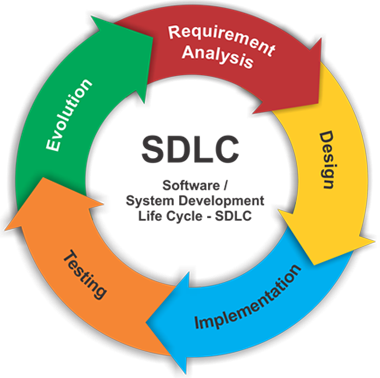
\includegraphics[width=0.5\textwidth]{img/lifecycle}		
			\caption{I 5 stati del ciclo di vita di un prodotto.}
		\end{figure} 
		
		Associare un sistema di \underline{\hyperref[qualita]{qualità}} al modello adottato, aiuta a perseguire conformità nel \underline{\hyperref[progetto]{progetto}} e \underline{\hyperref[maturita]{maturità}} nei processi.	Conoscere il ciclo di vita previsto di un prodotto, aiuta a valutarne preventivamente i tempi, i costi e i rischi. Esistono \underline{\hyperref[processo]{processi}} di ciclo di vita, che specificano le \textit{attività} da svolgere per abilitare le transizioni di stato nel ciclo di vita, e \underline{\hyperref[modelli]{modelli}} di ciclo di vita, che descrivono questi processi e come concorrono ad abilitare le specifiche transizioni. Per organizzare le attività dei processi implicati, è necessario identificare le dipendenze tra gli ingressi dell'uno e le uscite dell'altro in modo da fissare quindi l'ordinamento nel tempo e i criteri di attivazione e completamento.
	
		\subsection{CLASSIFICAZIONE DEI REQUISITI} \index{Classificazione dei requisiti} \label{classificazione}
		Ordinare i \underline{\hyperref[requirements]{requisiti}} in base agli attributi dei prodotti (quello che devono fare) e ai processi (come devono farlo). Guardo in generale i requisiti e li classifico in base a \textbf{cosa devo fare} con il prodotto (quindi ho dei requisiti funzionali) e \textbf{come devo farlo} (e quindi ho dei requisiti di vincolo).
		
		\subsection{CMMI}	\index{CMMI} \label{cmmi} %(slide 11) Set Lezione del 4/12 - Qualità di processo
		CMM (\textit{\underline{\hyperref[capability]{Capability}} \underline{\hyperref[maturity]{Maturity}} Model}) evoluto poi in CMMI (\textit{Capability Maturity Model Integration}) è un modello per la valutazione uniforme dei fornitori. \\
		\textit{Model} è l'insieme di criteri per valutare il grado di qualità (in scala assoluta) dei processi dell’azienda, mentre \textit{Integration} è l'architettura di integrazione delle diverse discipline (system, HW, SW) e tipologie di attività delle aziende.
		
		\subsection{CoCoMo}	\index{CoCoMo} \label{cocomo}
		\textit{Constructive Cost Model} è un modello algoritmico che stima le risorse necessarie esprimendone la misura in mesi/persona MP. 1 mese/persona sono 152 ore. [Per formule e il resto vedi slide 21/35-24/35]  
		
		\subsection{COESO} \index{Coeso} \label{coeso}
		Ciò che deve esserci e se non ci fosse mancherebbe. Sono quindi attività messe insieme a un dato scopo. \\
		Per quel che riguarda le componenti di un'\underline{\hyperref[architettura]{architettura}} possiamo dire che funzionalità "vicine" devono stare nella stessa componente e dato che la modularità spinge a decomporre il grande in piccolo, la ricerca di coesione fornisce un criterio di decomposizione. La coesione va massimizzata per ottenere maggiore manutenibilità e riusabilità, minor legame fra componenti e maggiore comprensibilità dell’architettura del sistema. Ci sono diversi tipi di buona coesione (la migliore è sempre quella che persegue \textit{information hiding}):
			\begin{itemize}
				\item \textbf{Funzionale}: quando le parti concorrono allo stesso specifico compito;
				\item \textbf{Sequenziale}: quando alcune azioni sono "vicine" ad altre per ordine di esecuzione ed è conveniente tenerle insieme;
				\item \textbf{Informativa}: quando le parti agiscono sulla stessa unità di informazione (la \underline{\hyperref[best]{best}} practice);
			\end{itemize}
		
		\subsection{COLLAUDO}	\index{Collaudo}	\label{collaudo}
		È l'atto formale di verifica di efficienza o di validità.  Ad esso segue il rilascio del prodotto e la fine della commessa.
		
		\subsection{COMMITTENTE} \index{Committente} \label{committente}
		Il suo compito è quello di identificare il prodotto da commissionare.
		
		\subsection{COMPONENTE} \index{Componente} \label{componente}
		Radice della composizione, ovvero non soltanto è una parte, ma è fatto per essere messo insieme.	
		
		\subsection{COMPORTAMENTO PREDICIBILE}	\label{comportamentopredicibile} %13 dicembre - verifica e validazione: analisi statica
		Ci interessa garantire comportamento predicibile del SW, ovvero che lo posso dire prima, perché non ci sia ambiguità. Elementi di vulnerabilità per garantire comportamento predicibile del SW:
		\begin{itemize}
			\item \textbf{Effetti laterali} (side-effect): la causa sono variabili condivise; la soluzione è incapsulazione.
			\item \textbf{Ordine}: di due importanti momenti:
			\begin{itemize}
				\item \textbf{elaborazione}, ovvero preparare le risorse logiche di cui il programma avrà bisogno al principio, ad esempio avere un po' di RAM, quindi preparare l'ambiente di esecuzione;
				\item \textbf{inizializzazione}, ovvero dichiarare le variabili prima di fare \textit{begin};
			\end{itemize}
			\item \textbf{Passaggio di parametro}: per valore e per riferimento (ricordo che in Java le variabili vengono passate ad una funzione facendone una copia e ricordare esempio dello swap che non fa effettivamente lo scambio). %slide 8/30
		\end{itemize}
		
		
		\subsection{COMPUTATIONAL THINKING} \index{Computational thinking} \label{computational}
		L'insieme dei processi mentali coinvolti nella formulazione di un problema e della sua soluzione in modo tale che un umano o una macchina possa effettivamente eseguire. [Aumentare abilità e sfide proporzionalmente].
		
		
		\subsection{CONFIGURAZIONE} \index{Configurazione} \label{configurazione}
		Indica le parti di un prodotto software e come esse vengono messe insieme.
		
		
		\subsection{CONSIDERAZIONI PRAGMATICHE}	\label{pragmatico}
		L’efficacia dei metodi di verifica è funzione della qualità di strutturazione del codice. La verifica di un programma relaziona frammenti di codice con frammenti di specifica.
		
		
		\subsection{CONSUNTIVO} \index{Consuntivo} \label{consuntivo} 
		Rendiconto dei risultati di un dato periodo di attività di un ente o di un'impresa. Si stima verso la fine.
		Esiste:
			\begin{itemize}
				\item consuntivo di periodo: ogni azione in questo periodo chiede nuova pianificazione sul rimanente (il prodotto è Pianificazione del residuo);
				\item preventivo a finire: conseguente al consuntivo di periodo;
			\end{itemize}
		  
		
		\subsection{CONTROLLO} \index{Controllo} \label{controllo}
			\subsubsection{Di Versione}  \label{controllodiversione}
			Gestione della storia di un prodotto.
			\subsubsection{Di Configurazione}  \label{controllodiconfigurazione}
			Codice frammentato in parti [non vogliamo 2000 righe].
			
			
		\subsection{CONTROLLO DI QUALITÀ}	\index{Controllo di Qualità}	\label{controlloqualita} %slide 9/22 Set Qualità del software
		Controllo di Qualità (o \textit{Quality Assurance}) sono le attività del sistema qualità pianificate e attuate per assicurare che il prodotto soddisfi le attese. Si può fare in due modi:
		\begin{itemize}
			\item assaggiatore: ogni prodotto realizzato lo faccio valutare (non è la miglior soluzione perchè non vado a monte del problema, potrei sprecare risorse);
			\item \textbf{quality assurance}: perseguendo attivamente; o è uno sforzo collettivo. Bisogna avere un \textit{way of working} che mostrano fiducia e controllo a monte. Ma tutto questo deve avvenire in modo non invasivo. Conviene seguire uno \underline{\hyperref[standard]{standard}}.
		\end{itemize}	
		
		
		\subsection{CORRELATO} \index{Correlato} \label{correlato}
		Cose che c'entrano/ che riguardano.
		
		
		\subsection{CORRETTEZZA}	\index{Correttezza} \label{correttezza}
			\subsubsection{per costruzione}	\label{byconstruction}
			\textit{"By construction"} vuol dire avere strumenti oggettivi misurabili che ci dicono se stiamo andando bene. Con regole sono confidente su quello che ho fatto.
			\subsubsection{per correzione} \label{bycorrection}
			\textit{"Correctness by correction"} vuol dire provarci, cercando di sistemare pezzo per pezzo; non sappiamo quindi effettivamente se funziona.
			
		\subsection{COVERAGE}	\index{Coverage}	\label{coverage}
		Il \textit{fattore di copertura} è quanto la prova esercita il prodotto rispetto alla percentuale di:
		\begin{itemize}
			\item funzionalità esercitate come viste dall'esterno: \textit{copertura funzionale}
			\item logica interna del codice esercitata: \textit{copertura strutturale} (branch, condition)
		\end{itemize}	
		\textbf{Attenzione}: una copertura al 100\% non prova assenza di difetti e in ogni caso un 100\% può essere irraggiungibile.
			
			
		\subsection{CRITERI DI PROGRAMMAZIONE}	\index{Criteri di programmazione}	\label{criteriprog}
		Criteri di programmazione: %slide 10/30 13 dicembre - verifica e validazione: analisi statica
		i \textit{criteri}(ovvero norme fondanti) servono per riconoscere qui i principi che ho usato per fare incapsulazione e altre norme: 
		\begin{itemize}
			\item Architettura (\textit{\underline{\hyperref[progettazione]{design}}}) del codice;
			\item Separare interfaccia e implementazione: ciò rende bassissimo l'accoppiamento (il client non deve conoscere l'implementazione ma solo l'interfaccia che non deve cambiare);
			\item Massimizzare information hiding;
			\item Uso i tipi (se ci sono): devo fare operazioni il cui esito sia verificabile, sapendo i tipi;
		\end{itemize}	
		
		
		\subsection{CUSTOMER} \index{Customer} \label{customer}
		Primo elemento di un progetto. Comprende \underline{\hyperref[opportunity]{opportunity}} e \underline{\hyperref[stakeholder]{stakeholders}}; 
	
	
